\section{The Normal Distribution and $\chi^{2}$}
A great deal of practical geodesy consists in taking observations. The observed values are
real numbers. But they are not exact; they include “random” errors. In order to analyze
these values we take them to be continuous random variables. In distinction to a real
variable, a random variable is furnished with a probability distribution.

Allow us a quick review of the normal distribution, before we introduce $\chi^2$ for the
sum of squares of independent normals. The chance that a random X falls between a and b
is found by integrating the probability density p(x):
\begin{equation}
Prob(a\leq X \leq b) = \int^a_bp(x)dx.
\end{equation} 
\begin{figure}[h]
	\centering
	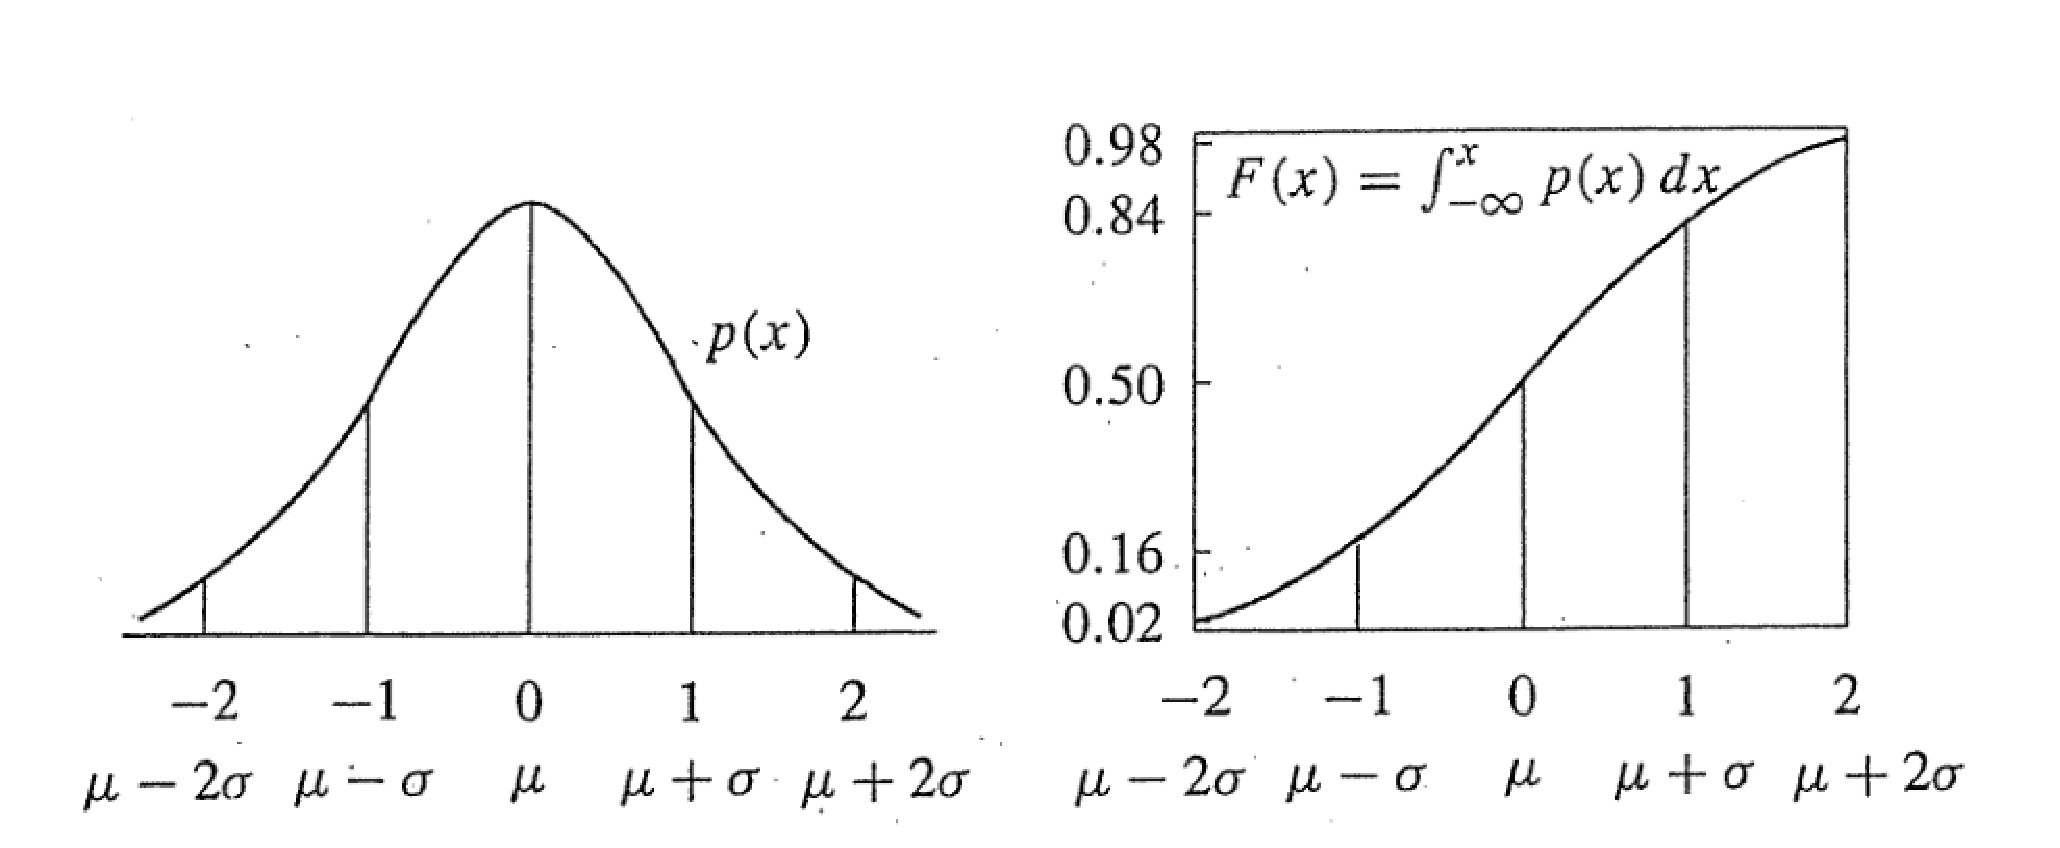
\includegraphics[width=0.7\linewidth]{TeX_files/Part02/chapter04/image/4-5}
	\caption{}
	\label{fig:4-5}
\end{figure}
Figure 4.5\; The normal distribution p(x)( bell-shaped) and its cumulative density F(x):
p(x) is given in (4.35)-(4.36) and there is no explicit formula for its integral F(x).

Roughly speaking, p(x)dx is the chance of falling between x and x + dx. Certainly
$p(x)\geq0$. If a and b are the extreme limits $-\infty$ and $\infty$, including all possible outcomes, the probability is necessarily one: 
\begin{equation}
Prob(-\infty < X < +\infty) = \int^{\infty}_{-\infty}p(x)dx=1.
\end{equation}
The most important density function is the normal distribution which is defined as
\begin{equation}
p(x)=\frac{1}{\sqrt{2\pi}\sigma}e^{-(x-\mu)/2\sigma^{2}}.
\end{equation}
Equation (4.35) involves the mean value $\mu$ and the standard deviation $\sigma$(which measures
the spread around the mean value). Often the two parameters are given the “standardized”
values $\mu=0$ and$\sigma$. Any normal distribution (4.35) can be standardized by the substitution $y=(x-\mu)/\sigma$. Then p(x) becomes symmetric around x = 0 and the variance is
$\sigma^2=1$:
\begin{equation}
Standard\, normal \qquad p(x)=\frac{1}{\sqrt{2\pi}}e^{-x^2/2}.
\end{equation}
The factor $\sqrt{2\pi}$ is included to make $\int p(x)dx=1$.
 
The bell-shaped graph of p(x) in Figure 4.5 is symmetric around the middle point
$x=\mu$. The width of the graph is governed by the second parameter $\sigma$— which stretches
the x axis and shrinks the y axis (leaving total area equal to 1). The axes are labeled to
show the standard case $\mu=0,\sigma=1$ and also the graph of p(x) for any other $\mu$ and $\sigma$.

We now give a name to the integral of p(x). The limits will be $-\infty$ and x, so the
integral F(x) measures the probability that a random sample is below x:
\begin{equation}
Prob(X\leq x)=\int^x_{-\infty}p(x)dx=cumulative density function F(x).
\end{equation}
F(x) accumulates the probabilities given by p(x), so dF(x)/dx = p(x). The reverse of
the integral is the derivative. The total probability is $F(\infty)=1$. This integral from
$-\infty$ to $\infty$ covers all outcomes.
\begin{table}
	Table 4.1\; One-dimensional normal distribution: Confidence intervals
	\centering
	\begin{tabular}{c c}
		\hline 
		Range of x & Probability \\ 
		\hline 
		$|x-\mu|\leq \sigma$  & 0.6827 \\  
		$|x-\mu|\leq 2\sigma$ & 0.9544 \\ 
		$|x-\mu|\leq 3\sigma$ & 0.9973 \\ 
		\hline
	\end{tabular}
\qquad
	\begin{tabular}{c c}
	\hline 
	Probability & Range of x \\ 
	\hline 
	0.50 &   $|x-\mu|\leq 0.674\sigma$\\
	0.95 &   $|x-\mu|\leq 1.960\sigma$\\
	0.99 &   $|x-\mu|\leq 2.576\sigma$\\
	\hline 
	\end{tabular}  	
\end{table}

Figure 4.5\; (right) shows the integral of the bell-shaped normal distribution. The middle point $x=\mu$ has $F=\frac{1}{2}$. By symmetry, there is a 50-50 chance of an outcome below the mean. The cumulative density F(x) is near 0.16 at $\mu-\sigma$ and near 0.84 at $\mu+\sigma$. The chance of falling in the interval $[\mu-\sigma,\mu+\sigma ]$ is 0.84 — 0.16 = 0.68. Thus 68\% of the outcomes are less than one deviation a from the center $\mu$.

Moving out to $\mu-1.96\sigma$ and $\mu+1.96\sigma$, 95\% of the area is in between, see Table 4.1. With $95\%$ confidence X is less than two deviations from the mean. Only one outcome in 20 further out (less than one in 40 on each side). This $95\%$ confidence interval is often taken as an indicator. When an observation is outside this interval, when it is more than $2\sigma$ away from $\mu$, we may accept that this happened with probability below 5\% or we may question whether the estimated values for $\mu$ and $\sigma$ are correct. 

Geodesy frequently sets the standard error further out, at $\mu+3\sigma$. The cumulative
density at that point is F = 0.9987. Thus the probability of a (one dimensional) sample
further than three standard deviations from the mean (above or below) is 2(1 - F) = 0.0027. Table 4.2 shows cumulative probabilities at important breakpoints.
\begin{table}
	Table 4.2 \;  Cumulative density function F(x) for the normal distribution
\centering
\begin{tabular}{c c c c c c c c}
	\hline 
	x & 0.0 & 0.5 & 1.0 & 1.5 & 2.0 & 2.5 & 3.0 \\ 
	\hline 
	F(x) & 0.5 & 0.6915 & 0.8413 & 0.9332 & 0.9773 & 0.9938 & 0.9987 \\ 
	\hline 
\end{tabular} 
\end{table}


The integral of p(x) from a to b is the probability that a random sample X will lie in
this interval:
\begin{equation*}
Prob(a\leq X \leq b)=Prob(X \leq b)-Prob(X \leq a)=F(b)-F(a).
\end{equation*} 
For a random variable X which is normally distributed with $\mu=1$ and $\sigma=2$ we have
\begin{equation*}
Prob(2\leq X \leq 3)=Prob(2<X<3)=F(\frac{3-1}{2}) - F(\frac{2-1}{2})
\end{equation*}
\begin{equation*}
\qquad\qquad\qquad=F(1)-F(\frac{1}{2})=0.8413-0.6915=0.1498.
\end{equation*}
If $x_1,...x_n$ are independent random variables each with mean $\mu$ and variance $\sigma^2_0$ , then $\hat{x}=\Sigma x_i/n$ is still normally distributed with mean $\mu$. The variance is reduced to $\sigma^2_0/n$.
\begin{table}
Table 4.3 \; $\chi^2$ with n = 2: Probability $K_2(c^2)$ that $x^2+y^2\leq c^2$\\
	\centering
\begin{tabular}{c c}
	\hline 
	c & $K_2(c^2)$ \\ 
	\hline 
	1 & 0.3935 \\ 
	2 & 0.8647 \\ 
	3 & 0.9889 \\ 
	\hline 
\end{tabular} 
\qquad
\begin{tabular}{c c}
	\hline 
	$K_2(c^2)$ & c \\ 
	\hline 
	0.90 & 2.146 \\ 
	0.95 & 2.448 \\ 
	0.99 & 3.035 \\ 
	\hline 
\end{tabular} 
\end{table}


	\subsection{Two-Dimensional Normal Distribution}
	In two dimensions we have probability densities p(x,y). Again the integral over all possibilities, $-\infty<x<\infty$ and $-\infty<x<\infty$, is 1. The normal distribution is always of the greatest importance, and we write the standardized form first. The mean is $\mu=(0,0)$ and the 2 by 2 covariance matrix is $\Sigma= I$:
	\begin{equation}
	p(x,y)=\frac{1}{2\pi}e^{-(x^2+y^2)/2}
	\end{equation}
	The M-file twod generated the 100 points (x,y) in Figure 4.6 in accordance with this
	two-dimensional distribution. (You can obtain your own different set of 100 points.) The
	figure shows the circle of radius $2\sigma=2$ around the mean. In the two-dimensional normal distribution , only 86.47\% of the sample points are expected to be in this circle. This is because $\iint_{x^2+y^2<4}p(x,y)dxdy=.8647.$ We count 16 points outside the circle in our sample.
	
	Table 4.3 shows the corresponding numbers for the circles of radius $\sigma$ and $3\sigma$. The squared distance $s=x^2+y^2$ is governed by a $\chi^2_2$ distribution, which has the simple form $p2(s)=\frac{1}{2}e^{-s/2}$ in (4.41). The table also shows the multiples of a that will give 90\%, 95\%, and 99\% confidence intervals around the mean $\mu$(assuming we know $\mu$).
	
	We get the marginal distribution of y when we integrate over all x:
	\begin{equation}
	M(y)=\int^\infty_{-\infty}p(x,y)dx.
	\end{equation}
	In this instance M(y) is simply the one-dimensional normal distribution for y. That is
	because p(x,y) in (4.38) separates into a product p(x)p(y). The variables x and y are
	uncorrelated; the covariance matrix $\Sigma$ is diagonal. But certainly we meet many situations in which correlation is present and $\Sigma$ is not diagonal. This highly important idea is defined and developed in Section 4.5.1. We give here the normal distribution when the covariance matrix $\Sigma$ has diagonal entries $\sigma^2_x$ and $\sigma^2_y$ and off-diagonal entry $\Sigma_{12}=\Sigma_{21}=\sigma_{xy}$:
	\begin{equation}
	Bivariate\, normal \quad 
	p(x,y)=\frac{1}{2\pi\sqrt{|\Sigma|}}e^{-[x,y]\Sigma^{-1}[x,y]^{T/2}}.
	\end{equation}
	If the mean is moved from (0,0) to $(\mu_x,\mu_y)$, then replace x and y by $x-\mu_x$ and $y-\mu_y$.	
	\begin{figure}[h]
		\centering
		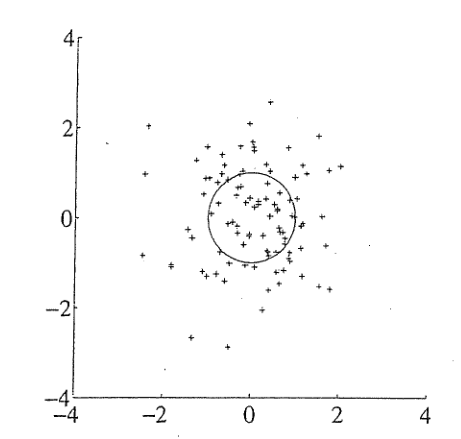
\includegraphics[width=0.7\linewidth]{TeX_files/Part02/chapter04/image/4-6}
		\caption{Figure 4.6\;The two-dimensional normal distribution and the circle of radius 1$\sigma$}
		\label{fig:4-6}
	\end{figure}
	
	\subsection{$\chi^2$ Distribution}
	Next we investigate the probability distribution for the sum of squares of the Gaussian
	random variables $x_1,...,x_n$:
	\begin{equation*}
	Random\, variable\,“chi-squared”\quad
	\chi^2_n=x^2_1+x^2_2+...+x^2_n.
	\end{equation*}
	We assume that the $x_i$ are independent and normally distributed with $\mu=0$ and $\sigma=1$.
	The random variable $\chi^2_n$ has a geometrical interpretation: $\chi^2_n$ is the squared distance from
	the origin to a point with coordinates $(x_1,...,x_n)$.
	
	In Example 4.8 we derive the density function for $x=\chi^2_1$ but already now we want
	to present the general expression for $x=x^2_1+x^2_2+...+x^2_n$ (and n = 2 is especially nice):
   \begin{equation}
   p_n(x)=\frac{1}{2^{n/2}\Gamma (n/2)}x^{(n/2)-1}e^{-x/2},
   \quad x\geq 0.
   \end{equation}
   For small values of n this $\chi^2_n$ distribution is strongly unsymmetric. Its mean value is $\mu=n$.
   \begin{equation}
   \mu=E{\chi^2_n}=\frac{1}{2^{n/2}\Gamma (n/2)}\int^{\infty}_0 xe^{-x/2}x^{n/2-1}dx =\frac{1}{2^{n/2}\Gamma (n/2)}\int^{\infty}_0 e^{-x/2}x^{n/2}dx
   \end{equation}
   \begin{equation*}
   \qquad =\frac{1}{2^{n/2}\Gamma (n/2)}\Gamma (1+n/2)2^{1+(n/2)}=\frac{(n/2)\Gamma (n/2)2^{1+(n/2)}}{2^{n/2}\Gamma (n/2)}=n.
   \end{equation*}
	Similarly we calculate the variance around the mean $\mu=n$ as $\sigma^2=2n$:
	\begin{equation}
	\begin{split}
	\sigma^2(\chi^2_n)&=\frac{1}{2^{n/2}\Gamma (n/2)}\int^{\infty}_0 xe^{-x/2}x^{n/2-1}dx-(mean)^2 \\
	&=\frac{1}{2^{n/2}\Gamma (n/2)}\Gamma (2+n/2)2^{2+(n/2)}-n^2 \\
	&=\frac{(1+n/2)(n/2)\Gamma (n/2)2^{2+(n/2)}}{2^{n/2}\Gamma (n/2)}-n^2\\
	&=(2+n)n-n^2=2n.
	\end{split}	
	\end{equation}

	\begin{figure}[h]
		\centering
		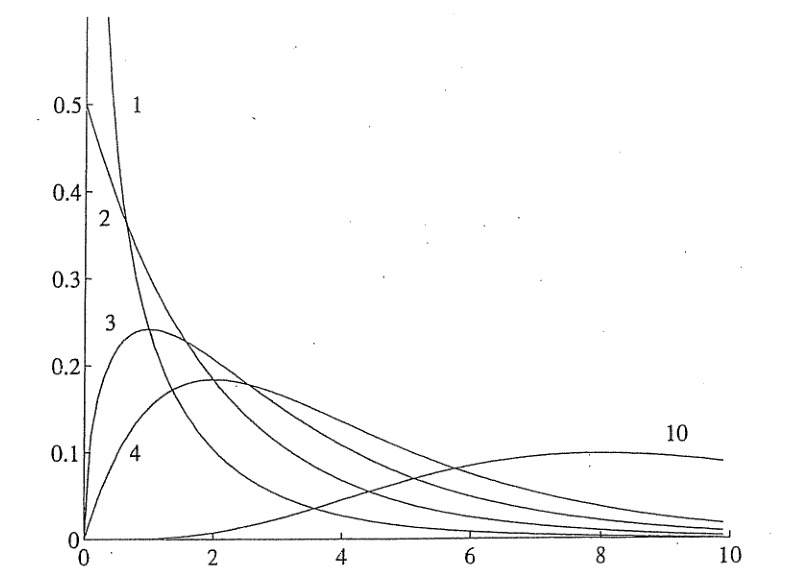
\includegraphics[width=0.7\linewidth]{TeX_files/Part02/chapter04/image/4-7}
		\caption{Figure 4.7\; Probability density $p_n(\chi^2)$ with n = 1,2,3,4,10 degrees of freedom}
		\label{fig:4-7}
	\end{figure}	
	For $n\longrightarrow\infty$, the distribution of $\chi^2_n$ tends to the normal distribution with mean 1 and variance $\sigma^2=2/n$. Figure 4.7 shows $p_n(x)$ for n =1,2,3,4,and 10.
	
	Example 4.8 Derivation of the $\chi^2_n$ distribution (4.41). Start with $x^2_1$:
	\begin{equation*}	
	\begin{split}
	Prob(x<\chi^2_n<x+dx)&= Prob(\sqrt{x}<x_1<\sqrt{x+dx})+Prob(-\sqrt{x+dx}<x_1<-\sqrt{x})\\
	&=Prob(\sqrt{x}<\lambda_1<\sqrt{x+dx}).
	\end{split}
	\end{equation*}
	We expand $\sqrt{x+dx}$ into a Taylor series $\sqrt{x}+dx/2\sqrt{x}$+ ... to obtain
	\begin{equation*}	
	\begin{split}
	2Prob(\sqrt{x}<x_1<\sqrt{x+dx})&\approx Prob(\sqrt{x}<x_1<\sqrt{x}+\frac{dx}{2\sqrt{x}})\\
	&\approx \frac{2}{\sqrt{2\pi}}e^{-x/2}\frac{dx}{2\sqrt{x}}=\frac{1}{\sqrt{2\pi x}}e^{-x/2}dx.
	\end{split}
	\end{equation*}
	This informal argument agrees with (4.41) since $\Gamma (\frac{1}{2})=\sqrt{\pi}$:
	\begin{equation}
	\chi^2_1\,distribution \qquad p_1(x)=\frac{1}{\sqrt{2\pi x}}e^{-x/2} \quad for\,x>0.
	\end{equation}
	Alternatively one could start from the cumulative distribution for $\chi^2_n$:
	\begin{equation*}
	Prob(\chi^2_1<x)= Prob(-\sqrt{x}<\chi_1<\sqrt{x})=2F(\sqrt{x})-1.
	\end{equation*}
	Then formally $p_1(x)$ is the derivative, and we recover (4.44):
	\begin{equation*}
	p_1(x)=\frac{d}{dx}(2F(\sqrt{x})-1)=\frac{1}{\sqrt{x}}\frac{1}{\sqrt{2\pi}}e^{-x/2}.
	\end{equation*}
	We intend to prove by induction the distribution for $x=\chi^2_1+ ... +\chi^2_n$:
	\begin{equation}
	p_n(x)=\frac{1}{2^{n/2}\Gamma (n/2)}x^{(n-2)/2}e^{-x/2} \quad for\,x\geq 0.
	\end{equation}
	
	Assume that equation (4.45) is valid for the indices 1,2,...,n. Then $\chi^2_{n+1}=\chi^2_n+\chi^2_1$. Again$\chi^2_n$ and $\chi^2_1$ are independent. Now we need the convolution theorem for probability densities: The probability density function of the sum of two independent random variables is the convolution of their probability density functions:
	\begin{equation}
	\begin{split}
	p_{n+1}(x) & =\int^x_0 p_n(y)p_1(x-y)dy = c_n\int^x_0 y^{(n/2)-1}e^{-y/2}\frac{e^{-(x-y)/2}}{\sqrt{x-y}}dy \\
	&=c_ne^{-x/2}\int^x_0\frac{y^{(n/2)-1}}{\sqrt{x-y}}dy \\
	&=c_ne^{-x/2}x^{(n-1)/2}\int^x_0(\frac{y}{x})^{(n/2)-1}(1-\frac{y}{x})^{-1/2}d(\frac{y}{x})\\
	&=C_nx^{(n-1)/2}e^{-x/2}.	
	\end{split}
	\end{equation}
	We determine the constant $C_n$ so that the total probability is 1:
	\begin{equation*}
	\int^{\infty}_0p_{n+1}(x)dx=C_n\int^{\infty}_0x^{(n-1)/2}e^{-x/2}dx=1.
	\end{equation*}
	Replacing x/2 by t, the integral becomes the gamma function:
	\begin{equation*}
	C_n2^{(n+1)/2}\Gamma(\frac{n+1}{2})=1.
	\end{equation*}
	Bubstituting for $C_n$, equation (4.46) agrees with (4.45) for all positive integers n.
	
	In many applications the cumulative function $K_n(x)$is more useful than $p_n(x)$ itself:
	\begin{equation}
	K_n(x)=Prob(\chi^2_n\leq x)=\int^x_0p_n(t)dt.
	\end{equation}
	$K_n(x)$ gives the probability that the square sum of n normally distributed random variables $x_i$ is smaller than a given number x. This function is tabulated for various values
	of n. Without the factor $\frac{1}{(2^{n/2}\Gamma (n/2))}$, $K_n(x)$ is called the incomplete gamma function.
	
	Often one encounters distribution functions closely related to $\chi^2$. For example if $X=y^2_1 + ... +y^2_n$ with $E{y_i}=0$ and $E{y^2_i}=\sigma^2$ then $X=\sigma^2\chi^2_n$. We will also meet random variables of the form
	\begin{equation*}
	\begin{split}
	&\frac{1}{n}X=\frac{1}{n}(y^2_1 + ... +y^2_n)\\
	&\sqrt{X}=\sqrt{y^2_1 + ... +y^2_n}\\
	&\sqrt{\frac{1}{n}X}=\sqrt{\frac{1}{n}(y^2_1 + ... +y^2_n)}
	\end{split}
	\end{equation*}
	All these variables have density distributions related to $p_n(x)$. We gather them in Table 4.4.
	
	Statistical test theory assumes that we can present two clear-cut alternative hypotheses. In
	geodesy this is seldom possible. So instead the concept of confidence regions is much more
	used, and that brings the x 2 distribution into play.
	\begin{table}
		Table 4.4 Random variables and their probability densities\\
		\centering
		\begin{tabular}{c c}
			\hline 
			Random variable & Probability density when $y_i$ are $N(0,\sigma^2)$ \\ 
			\hline 
			$X=\sum^n_{i=1}y^2_i$ & $\frac{1}{\sigma^2}p_n(\frac{y}{\sigma})=\frac{1}{2^(n/2)\Gamma(n/2)\sigma^n}y^{(n/2)-1}e^{-y/(2\sigma^2)}$ \\ 
			$\frac{1}{n}X=\frac{1}{n}\sum^n_{i=1}y^2_i$ &  
			$\frac{n}{\sigma^2}p_n(\frac{ny}{\sigma})=\frac{(n/2)^{n/2}}{\Gamma(n/2)\sigma^n}y^{(n/2)-1}e^{-ny/(2\sigma^2)}$ \\ 
			$\sqrt{X}=\sqrt{\sum^n_{i=1}y^2_i}$ &
			$\frac{2y}{\sigma^2}p_n(\frac{y^2}{\sigma^2})=\frac{1}{2^(n/2)\Gamma(n/2)\sigma^n}y^{n-1}e^{-y^2/(2\sigma^2)}$  \\ 
			$\sqrt{\frac{1}{n}X}=\sqrt{\frac{1}{n}\sum^n_{i=1}y^2_i}$ & 
			$\frac{2ny}{\sigma^2}p_n(\frac{ny^2}{\sigma^2})=\frac{2(n/2)^{n/2}}{\Gamma(n/2)\sigma^n}y^{n-1}e^{-ny^2/(2\sigma^2)}$  \\ 
			\hline 
		\end{tabular} 
	\end{table}
	
	
	In particular, the random variable $(n-1)\hat{\sigma}^2/\sigma^2_0$ using the sample variance
	$\hat{\sigma}^2=\frac{1}{n-1}\Sigma(x_i-\hat{x})^2$ follows a $\chi^2$ distribution with n — 1 degrees of freedom.
	
	Remember $K_n(x)$ is a cumulative probability. When this probability is fixed at some
	specific value $K_n(x)=P\%$ the corresponding value for x is known as the P\%-fractile.
	For the $\chi^2$ distribution with n degrees of freedom the P\%-fractile is represented by the
	symbol $\chi^2_{n,P}$. Values of $\chi^2_{n,P}$ are given in Table 4.5.
	
	By means of the $\chi^2$ distribution and the estimated variance $\hat{\sigma}^2$ we can derive confidence intervals for the (theoretical) variance $\sigma^2_0$. Estimates are usually denoted by a hat($\hat{}$).	Let the P\%-fractile of the $\chi^2$ distribution with n - 1 degrees of freedom be called $\chi^2_{n-1,P}$.
	
	Then
	\begin{equation*}
	Prob(\chi^2_{n-1,Q}<\frac{(n-1)\hat{\sigma}^2}{\sigma^2_0}<\chi^2_{n-1,P})=P-Q.
	\end{equation*}
	We solve this equation for $\sigma^2_0$ and obtain the (P - Q)\%-confidence interval for $\sigma^2_0$:
	\begin{equation}
	\frac{n-1}{\chi^2_{n-1,P}}\hat{\sigma}^2<\sigma^2_0<\frac{n-1}{\chi^2_{n-1,Q}}\hat{\sigma}^2.
	\end{equation}
	If we have w unknowns instead of 1, the number n — 1 changes to n - u.
	
	For the two-sided confidence interval $Q > 0$ and $P < 100$, we put Q = 100 — P.
	Then equation (4.48) becomes
	\begin{equation}
	\frac{n-u}{\chi^2_{n-u,P}}\hat{\sigma}^2<\sigma^2_0<\frac{n-u}{\chi^2_{n-u,(100-P)}}\hat{\sigma}^2.
	\end{equation}
	If the confidence is selected as 90\% then often this is split into two equal halves and one
	calculates the probability to get a lower and an upper limit.
	\begin{table}
	Table 4.5 Probabilities for one-sided P\%-fractiles of the $\chi^2$ distribution \\
	\centering
	\begin{tabular}{c c c c c c c c}
		\hline 
		n-u & 1\% & 5\% & 10\% & 50\% & 90\% & 95\% & 99\% \\ 

		1 & 0.00016 & 0.0039 & 0.016 & 0.5 & 2.7 & 3.8 & 6.6 \\ 
 
		2 & 0.020 & 0.103 & 0.211 & 1.4 & 4.6 & 6.0 & 9.2 \\ 

		3 & 0.115 & 0.352 & 0.584 & 2.4 & 6.3 & 7.8 & 11.3 \\ 

		4 & 0.30 & 0.71 & 1.06 & 3.4 & 7.8 & 9.5 & 13.3 \\ 
 
		5 & 0.55 & 1.15 & 1.61 & 4.4 & 9.2 & 11.1 & 15.1 \\ 
 
		6 & 0.87 & 1.64 & 2.20 & 5.3 & 10.6 & 12.6 & 16.8 \\ 

		8 & 1.65 & 2.73 & 3.49 & 7.3 & 13.4 & 15.5 & 20.1 \\ 
 
		10 & 2.56 & 3.94 & 4.87 & 9.3 & 16.0 & 18.3 & 23.2 \\ 

		20 & 8.3 & 10.9 & 12.4 & 19.3 & 28.4 & 31.4 & 37.6 \\ 

		30 & 15.0 & 18.5 & 20.6 & 29.3 & 40.3 & 43.8 & 50.9 \\ 

		40 & 22.2 & 26.5 & 29.1 & 39.3 & 51.8 & 55.8 & 63.7 \\ 

		50 & 29.7 & 34.8 & 37.7 & 49.3 & 63.2 & 67.5 & 76.2 \\ 
 
		100 & 70.1 & 77.9 & 82.4 & 99.3 & 118.5 & 124.3 & 135.8 \\ 
		\hline 
	\end{tabular} 	
	\end{table}
	
	
	Suppose an empirical standard deviation $\hat{\sigma}$ is determined on the basis of f degrees
	of freedom. We define a confidence interval (of confidence $1-\alpha$) for $\sigma_0$ through the probability conditions
	\begin{equation*}
	Prob(a\leq \sigma_0 <b)=1-\alpha \quad and \quad Prob(\sigma_0 <a)=Prob(\sigma_0 >b)=\alpha/2.
	\end{equation*}
	and we seek the limits a and b. Assume the original observations are normally distributed,
	so that $\chi^2_f=f\hat{\sigma}^2/\sigma^2_0$ and
	\begin{equation*}
	Prob(\chi^2_f\leq \chi^2_{f,\alpha/2})=\alpha/2 \quad and \quad 	
	Prob(\chi^2_f\leq \chi^2_{f,1-(\alpha/2)})=1-(\alpha/2).
	\end{equation*}
	Those combine into
	\begin{equation*}
	Prob(a\leq \sigma_0 <b)=1-\alpha
	\end{equation*}
	with
	\begin{equation*}
	a=\sqrt{\frac{f}{\chi^2_{f,1-(\alpha/2)}}}\hat{\sigma}=\gamma_a\hat{\sigma} 
		\quad and \quad 
	a=\sqrt{\frac{f}{\chi^2_{f,\alpha/2}}}\hat{\sigma}=\gamma_b\hat{\sigma}.	
	\end{equation*}
	
	\begin{table}
		Table 4.6 Limiting factors $\gamma_a$ and $\gamma_b$ for confidence interval with probability 0.95\\
		\centering
		\begin{tabular}{cccccccccc}
			\hline 
			m-n & 1 & 2 & 3 & 4 & 5 & 10 & 20 & 50 & 100 \\ 
			\hline
			$\gamma _a$ & 0.446 & 0.521 & 0.567 & 0.599 & 0.624 & 0.699 & 0.765 & 0.837 & 0.879 \\ 

			$\gamma _b$ & 31.9 & 6.28 & 3.73 & 2.87 & 2.45 & 1.76 & 1.44 & 1.24 & 1.16 \\ 
			\hline 
		\end{tabular} 
	\end{table}

	
	The factors $\gamma_a$ and $\gamma_b$  obviously depend on the confidence probability $1-\alpha$ and the number of degrees of freedom. The factors are shown in Table 4.6 for $1-\alpha=0.95$. This uses Table 4.5 which can be found in Abramowitz \& Stegun (1972), Table 26.8. For f = 5 we get $0.672\hat{\sigma}<\sigma_0<2.09\hat{\sigma}$.
	
	A common geodetic least-squares problem is the estimation of coordinates of control points
	for a network. Simultaneously we get a covariance matrix for the estimates. This leads
	to the construction of the confidence ellipse, see Section 4.9. We now ask what is the
	probability that the estimated point will lie within this confidence ellipse. $K_2(c^2)$ tells the	probability for the following inequality:
	\begin{equation*}
	Inside\, the\, confidence\, ellipse \qquad
	\frac{y^2_1}{\lambda^2_1}+\frac{y^2_2}{\lambda^2_2}<c^2.
	\end{equation*}
	The integral of $p_2(x)=\frac{1}{2\Gamma (1)}x^0e^{-x/2}$ gives the cumulative probability $K_2$:
	\begin{equation}
	K_2(c^2)= Prob(\chi^2_2<c^2)=\frac{1}{2}\int^{c^2}_0e^{-x/2}dx=1-e^{-c^2/2}.
	\end{equation}
	We indicated some values in Table 4.3.
	
	\subsection{F Distribution}
	The ratio of sums of squares is often encountered in geodetic practice. Any adjustment
	starts by introducing an a priori variance of unit weight, most often chosen as $\sigma^2_0=1$.
	Equation ( 4.79 ) estimates the a posteriori value $\hat{\sigma^2_0}=\|b-A\hat{x}\|^2/(m-n)$ of the same variance. We expect the ratio $\hat{\sigma^2_0}/\hat{\sigma^2_0}$ to be close to unity. A typical application will be shown in Section 7.8. In mathematical statistics this hypothesis is called the null hypothesis $H_0$. The aim of the test is to obtain an indication whether this ratio is significantly different from unity. The answer is given by the F density function.
	
	Let $x_1,...,x_m$ and $y_1,...,y_n$ be normally distributed independent random variables. We define K as the dimensionless quantity
	\begin{equation}
	\kappa =\frac{\frac{1}{m}\sum^{m}_{i=1}x^2_i}{\frac{1}{n}\sum_{j=1}^{n}y^2_i}=\frac{s/m}{t/n}.
	\end{equation}
	We want the probability $F_{mn}(x)$ that this fraction $\kappa$ is smaller than a given constant x.
	
	The $\chi^2$ probability densities for the individual sums s and t are
	\begin{equation*}
	p_m(x)=\frac{1}{2^{m/2}\Gamma(m/2)}x^{(m/2)/2}e^{-x/2} \quad and \quad
	p_n(x)=\frac{1}{2^{n/2}\Gamma(n/2)}x^{(n/2)/2}e^{-x/2}
	\end{equation*}
	After some calculations we get the final formula for this F distribution:
	\begin{equation}
	F_{mn}(x)=\frac{\Gamma((m+n)/2)}{\Gamma(m/2)\Gamma(n/2)}(\frac{m}{n})^{m/2} 
	\quad
	\frac{x^{(m-2)/2}}{(1+(m/n)x)^{(m+n)/2}}
	\end{equation}